\chapter{Thermodynamics}
\section{Kinetic theory - Ryan's lesson transcript}
If KE is dependent on temperature, whats the difference between a cold moving ball, and a hot stationary ball. This is because the former is about \textbf{microscopic}, but the latter is about \textbf{macroscopic}. 

Because it is not feasible to model the motion of every single molecules with newton's laws, it is more convenient to use probability.

\subsection{Probability distribution}
We are working with \textbf{continuous} probability distribution $P(x) $where $0 \leq P(x) \leq 1$. The area under the curve (let's say from $a$ to $b$, $b>a$) would be the probability of the number $n$ to be $a\leq n\leq b$

\subsection{velocity distribution}
let the velocity probability distribution be $g(v_x)$
\begin{equation}
    g(v_x)\propto \exp\bigg({\frac{-mv_x^2}{2k_B T}}\bigg)
\end{equation}

To find the proportionality constant, we have to normalise the distribution by integrating the distribution from -1 to 1, and setting the integral to 1.

\begin{equation}
    \int_{-\infty}^{\infty}A\exp\bigg({\frac{-mv_x^2}{2k_B T}}\bigg)dv_x = 1
\end{equation}
This is the case where $\alpha=m/2k_BT$ (see Math section). Hence,
\begin{equation}
    g(v_x)=\sqrt{\frac{m}{2\pi k_B T}}\exp\bigg({\frac{-mv_x^2}{2k_BT}}\bigg)
\end{equation} 

To find the average velocity, we just need to integrate 
\begin{equation}
    \langle v_x \rangle =\int_{-\infty}^{\infty}v_xg(v_x)dv_x=0
\end{equation}
HAHA sike it is 0 cos its velocity not speed.

\subsection{speed distribution}
Speed $v=\sqrt{v_x^2+v_y^2+v_z^2}$ can be represented as the distance between the origin and a point in the velocity space.
\begin{figure}[H]
    \centering
    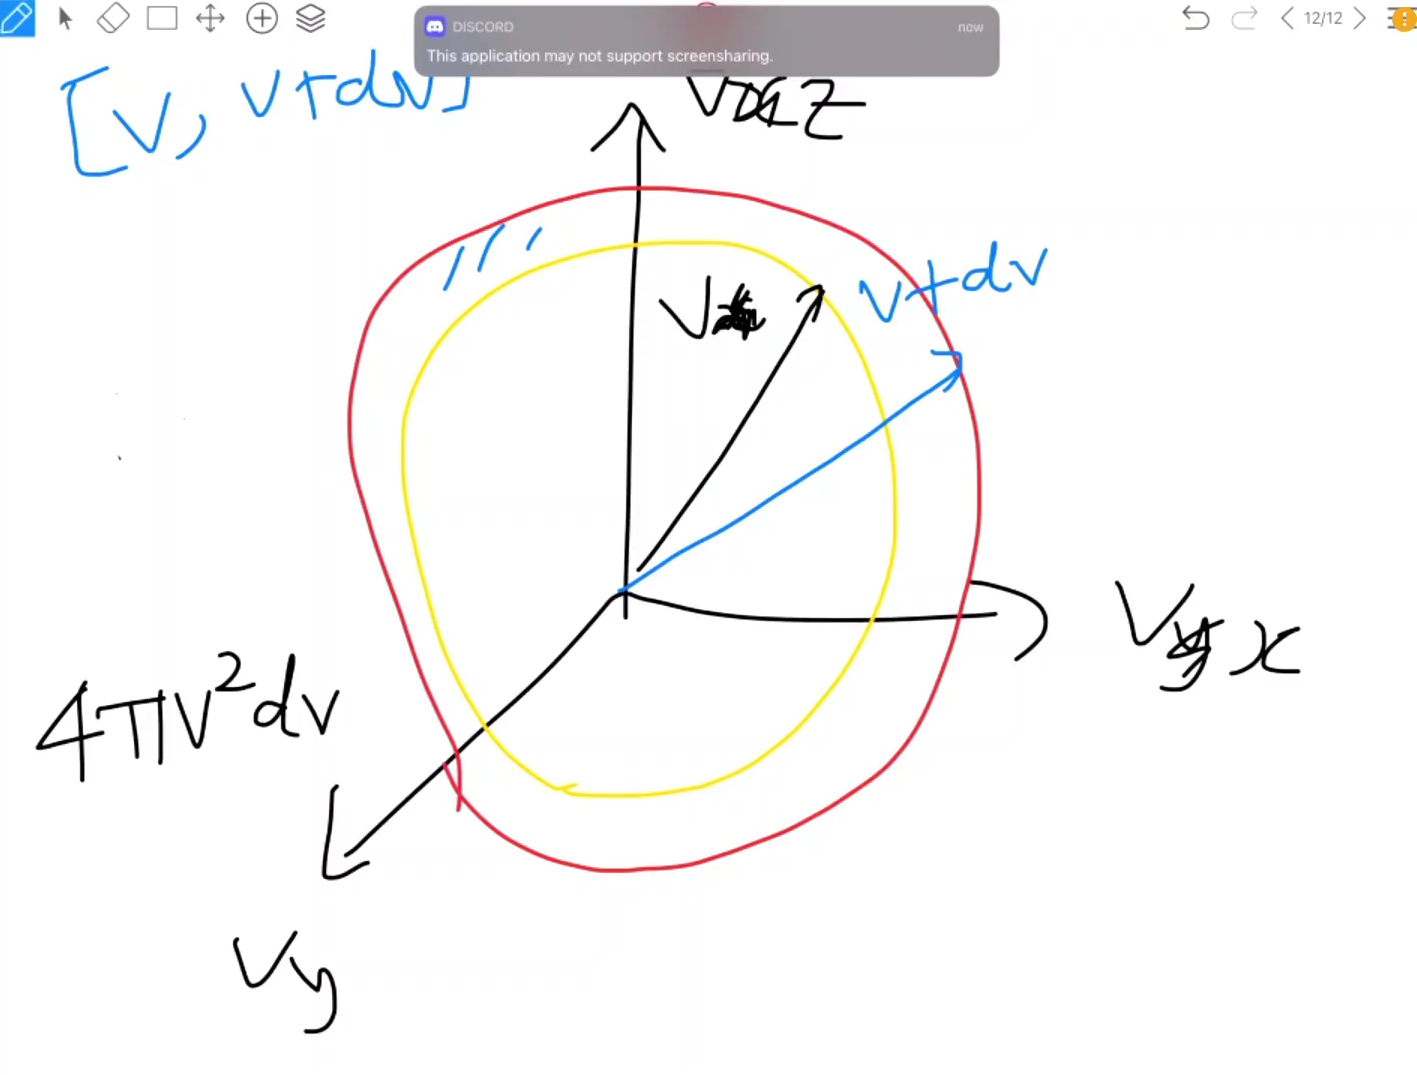
\includegraphics[width=0.5\linewidth]{velocity space.png}
    \caption{beautiful drawing by Ryan}
    \label{<label>}
\end{figure}
The volume enclosed, $V=4\pi v^2 dv$, between the red and yellow circle, multipled by the probability of the particles moving in that region, denotes the particles with speed $v \leq v_p \leq v+dv$. The speed probability distribution is then given by
\begin{equation}
    f(v)dv\propto v^2 \exp \bigg({\frac{-mv^2}{2k_B T}}\bigg)dv
\end{equation}

Integrating, we get
\begin{equation}
    f(v)=\frac{4}{\sqrt{\pi}}\bigg(\frac{m}{2 k_B T}\bigg)^\frac{3}{2} v^2 \exp\bigg({\frac{-mv^2}{2k_BT}}\bigg)
\end{equation}

Average speed:
\begin{equation}
    \langle v \rangle =\sqrt{\frac{8k_BT}{\pi m}}
\end{equation}

Root mean squared velocity: 
\begin{equation}
    \langle v^2 \rangle =\frac{3k_BT}{m} = \langle v_x^2\rangle + \langle v_y^2\rangle + \langle v_z^2\rangle
\end{equation}

Most probable speed: $df/dv=0$
\begin{equation} 
    v=\sqrt{\frac{2k_BT}{m}}
\end{equation}

Note: $m$ stand for the \textbf{molar mass} lmao not the actual mass of all the gas molecules. 

\subsection{Equipartition theorem}
Every degree of freedom will contribute $k_B T/2$ to the internal energy. 
\begin{equation}
    U=\frac{f}{2}k_BT
\end{equation}

More rigorous form: Each quadratic mode with energy in the form of $E=\alpha x^2$, where $x$ can be position or velocity, contributes $k_BT/2$ to the internal energy (so its not really about degree of freedom). It just so happens that both rotational and translational energy are $\propto v^2, \omega^2$

\section{Ideal gas law}
\begin{equation}
    p=\frac{1}{3}n m \langle v^2 \rangle
\end{equation}
where $n$ is the number of molecules per unit volume. and $m$ is the mass of the molecules.

\section{First Law of thermodynamics}
The first law of thermodynamics state that:
\begin{equation}
    \Delta E= \Delta Q + W
\end{equation}
Since there is a plus sign in front of $W$, it must mean \textbf{work done on the gas}.
The differntial form of the the equation above is
\begin{equation}
    dE=dQ+dW
\end{equation}
where $dQ$ and $dW$ are called \textbf{inexact differential} since they are path dependent (and not state dependent)quantities.

On the other hand, $E$ is a state dependent quantity (depends on both temperature, $T$ and volume, $V$). Hence, a small change in $E$ ($dE$) can also be written as
\begin{equation}
    dE(T,V)=\bigg(\frac{\partial E}{\partial T}\bigg)_V dT+\bigg(\frac{\partial E}{\partial V}\bigg)_T dV
\end{equation}
\begin{mybox}{gray}{Molar specific heat at constant \textbf{volume} and \textbf{pressure}}
    Molar specific heat:
    \begin{itemize}
        \item at constant \textbf{volume}
              \begin{equation}
                  C_V=\bigg(\frac{\partial Q}{\partial T}\bigg)_V=\bigg(\frac{\partial E}{\partial T}\bigg)_V
              \end{equation}
              Proportionality factor between heat supplied and temperature change of a system at constant volume
        \item at constant \textbf{pressure}
              \begin{equation}
                  C_p
                  =\bigg(\frac{\partial Q}{\partial T}\bigg)_p
                  =\bigg(\frac{\partial (E-W)}{\partial T}\bigg)_p
                  =\bigg(\frac{\partial E}{\partial T}\bigg)_p+
                  p\bigg(\frac{\partial V}{\partial T}\bigg)_p
              \end{equation}
    \end{itemize}
    (the plus sign in front of the work is because $dQ=dE-dW$, and $dW=-pdV$. This is before when volume of gas decreases, work must be done \textbf{on} it, increasing its internal energy).
    \begin{flushleft}
        Since $\big(\frac{\partial V}{\partial T}\big)$ at constant pressure is essentially $\frac{nR}{p}$, the second term reduces to just $nR$.
    \end{flushleft}

    $$\boxed{\therefore C_p=C_V+nR}$$
    This shows that it takes more heat to increase temperature for an isobaric process. This is because extra energy is needed to offset those used when the gas does work by expanding.

    This relationship can actually be derived through many other methods as well. But just need to remember
    \textbf{first law of thermodynamics}, \textbf{internal energy's dependence on both temperature and volume}, as well as the fact that \textbf{heat capacity is a proportionality factor between heat input and change in temperature (internal energy)}, then shld be okay :)

\end{mybox}
\section{Quasi-static process}
\textbf{Definition}: A thermodynamic process that happens slowly enough for the system to remain in internal \textbf{thermodynamic equilibrium} (no tendency for the state of a system to change spontaneously).
\subsubsection{Assuming a quasi-static process}
I think for most questions that talk about isochoric, isothermal and isobaric processes, the process is assumed to be quasi-static. This is because to be isothermal, isochoric or isobaric throughout the processes, you must be able to state the temperature, pressure and volume of the system at each step, which is possible only if the system is in equilibrium continuously.

\subsubsection{If process is not quasistatic}

If the question is about adiathermal process (according to Blundell, if the process is both adiathermal [without the flow of heat] and reversible, it's called adiabatic), the process can be carried out both quasi-statically and non quasi-statically. If the process is not quasi-static , we can no longer use the equation for various thermodynamic processes to solve the question. However, it is still possible to solve such questions using \textbf{conservation of energy.}

\begin{mybox}{green}{Quasi-static (reversible) process (my own interpretation)}
    If a gas changes state from A to B, it is only quasi-static if the intermediate states are all in thermodynamic equilibrium. Work done by isothermal / isochoric / isobaric processes are calculated with the assumption that processes are quasi-static (because infinitely small increments of change represent a continuous function).

    \begin{flushleft}
        E.g. If the process involves adding or removing weights from a piston (with gas beneath it), and the piston settles into a new equilibrium position, such a process is not quasi-static because the temperature / pressure / volume of the intermediate state is unknown (not in equilibrium). (Or when the process happens too fast such that there's insufficient time for the gas to settle into equilibrium)
    \end{flushleft}

\end{mybox}

Also err i am not exactly sure why but for an adiabatic process,
\begin{equation}
    dQ=\bigg(\frac{\partial Q}{\partial V}\bigg)_p dV + \bigg(\frac{\partial Q}{\partial p}\bigg)_V dp=0
\end{equation}

\section{Heat engines lol}
A Carnot engine (engine is defined as something that converts heat into work, 2 adiabats + 2 isotherms). We can prove by analysing each individual process that:
\begin{equation}
    \frac{Q_h}{Q_l}=\frac{T_h}{T_l}
\end{equation}
Efficiency a carnot engine (turns heat into work) is defined as the ratio of work done to the heat input, hence $\eta=\frac{W}{Q_h}$, where $W=Q_h-Q_l$, as the process is cyclic and there is no change in internal energy.

\begin{flushleft}
    However, for a refrigerator (engine run in reverse), the efficiency is defined as a different way. It is instead
    \begin{equation}
        \eta=\frac{Q_l}{W}
    \end{equation}
    It makes sense because efficiency in this case means the amount of heat you can \textbf{remove} from a refrigerator when the engine does a certain amount of work. (similar for a heat pump, where the engine does work to pump heat instead of remove heat).
\end{flushleft}

\begin{mybox}{gray}{Clausius' inequality}
    Clausius' inequality states that for any closed loop,
    \begin{equation}
        \oint \frac{dQ}{T} \leq 0
    \end{equation}
    and equality must hold for reversible reactions.
\end{mybox}

\section{Second law of thermodynamics}
Entropy is a state function, and it is defined as such
\begin{equation}
    S(B)-S(A)=\int_A^B \frac{dQ}{T}
\end{equation}
This is because the closed loop integral of $\frac{dQ}{T}=0$ for ideal, reversible process, showing that this quantity is path independent (state dependent just like electric potential.)

\begin{flushleft}
    For an adiabatic process, $dQ=0$. Hence, there is no change in entropy for an adiabaticprocess (\textbf{isentropic})
\end{flushleft}
\section{Modes of heat transfer}